\begin{figure}[h]
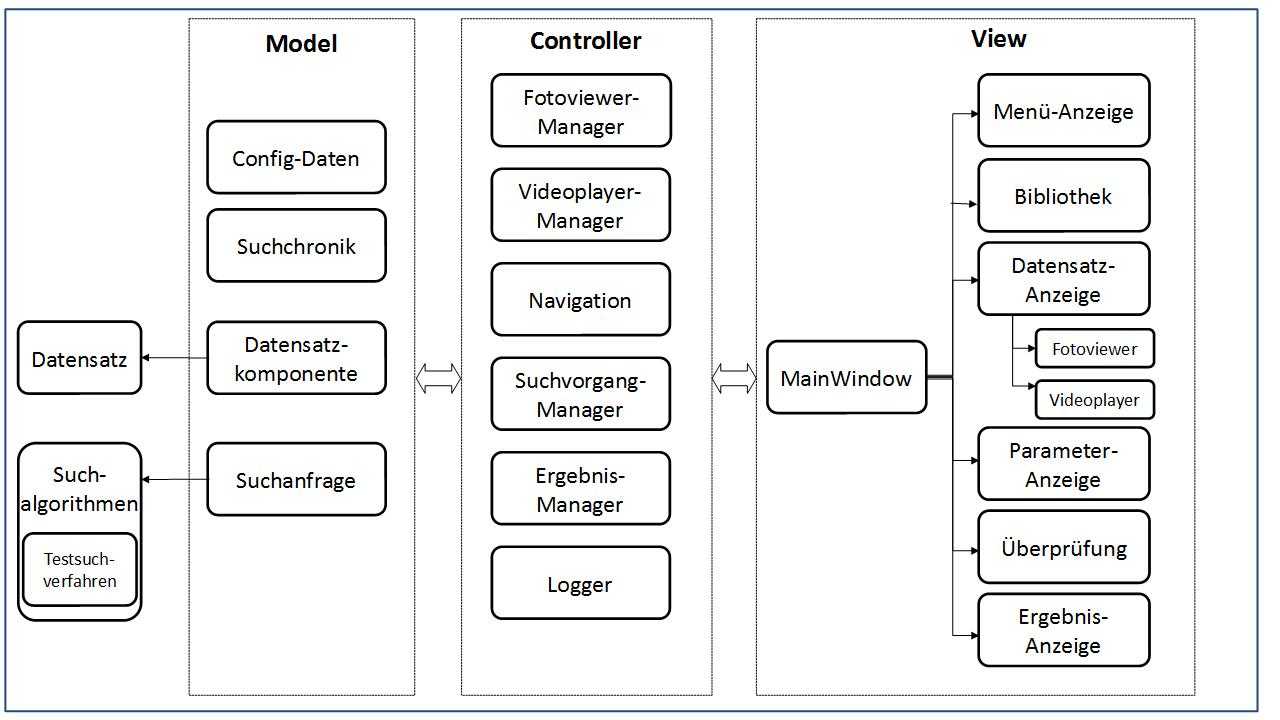
\includegraphics[width=1\linewidth]{img/sysmodell}
\caption{Systemmodell}
\label{fig:systemmodell}
\end{figure}
\vspace{10pt}

Die Grundstruktur des Programms folgt dem Prinzip der \glslink{Model-View-Controller}{MVC}-Architektur. Die Unterteilung der Submodule in Model, View und Controller ermöglicht eine leichte Modifikation und Erweiterung.

\begin{itemize}
\item Datensatz\newline
Die Bilder und Videos bilden eine Grundlage der Anwendung, außerdem kann ein Datensatz \glslink{Annotation} {Annotationen} enthalten.
\item Datensatzschnittstelle\newline
Die Datensatzschnittstelle bietet sowohl der Anwendung als auch den \gls{Suchverfahren} einen einheitlichen Zugriff auf die hinterlegten Daten. Diese Schnittstelle wird von der Datensatzkomponente implementiert.
\item \glslink{Suchverfahren}{Suchalgorithmen}\newline
Verschiedene austauschbare inhaltsbasierte \glslink{Suchverfahren}{Suchalgorithmen}. Unter einer wohldefinierten Schnittstelle kann CoBaB die Algorithmen verwenden.
\item Suchschnittstelle\newline
Die Suchschnittstelle ermöglicht eine einheitliche Verwendung der \glslink{Suchverfahren}{Suchalgorithmen}. Jedes \gls{Suchverfahren}, insbesondere das Testsuchverfahren, implementiert diese Schnittstelle.
\end{itemize}

\subsection{Model}
\begin{itemize}
\item Config-Daten\newline
Die Konfigurationsdaten passen die Anwendung an die Präferenzen des Benutzers an: Die gewählte Sprache und die Aktivierung bzw. Deaktivierung des Benachrichtigungstons werden gespeichert und beim erneuten Starten der Anwendung als Voreinstellung gesetzt. Außerdem wird eine Hilfe-Datei gespeichert.
\item Datensatzkomponente\newline
Die Datensatzkomponente implementiert die Datensatzschnittstelle, um auf die Bilder bzw. Videos zuzugreifen.
\item Suchanfrage\newline
Die Suchanfrage ist der Input für das Verfahren. Die Anwendung generiert eine Suchanfrage, die aus gewählter Suchvorlage, gewünschtem \gls{Suchverfahren}, den Suchparametern und dem Suchraum besteht. Der Suchraum ist durch den Datensatz festgelegt, in dem gesucht werden soll.
\item \gls{Suchchronik}\newline
Die \gls{Suchchronik} speichert die letzten Suchergebnisse, um sie anzeigen zu lassen. Außerdem speichert sie \gls{Lesezeichen} für spezielle Ergebnisse.
\end{itemize}

\subsection{View}
\begin{itemize}
\item MainWindow \newline
Das MainWindow ist das Hauptfenster von CoBaB. Es zeigt die \glspl{Widget} an.

\item Menü-Anzeige \newline
Das Menü beinhaltet Bequemlichkeitsfunktionen wie \textbf{Datei}, wo zusätzlich das Beenden des Programms und die Datensatzauswahl ermöglicht wird, \textbf{Sprachauswahl}, \textbf{Hilfe}, wo es Informationen über das Programm gibt oder Anweisungen zum Benutzen der Anwendung, \textbf{\gls{Suchchronik}} mit gespeicherten früheren Suchen, \textbf{\gls{Lesezeichen}}, die der Benutzer selbst aus seinen Suchergebnissen erstellt.

\item Bibliothek \newline
Die Bibliothek ist beim Starten des Programms zu sehen. Anfangs ist nur eine voreingestellte Auswahl an Datensätzen zu sehen. Jedes mal beim erneuten Öffnen werden die zuletzt genutzten Datensätze angezeigt. Man kann entweder einen Datensatz aus den angezeigten wählen oder über einen Auswahl-\gls{Dialog} einen neuen suchen.

\item Datensatzanzeige \newline
Nach der Auswahl eines Datensatzes wird der Inhalt angezeigt. Dem Datensatz entsprechend wird der Fotoviewer oder der Videoplayer integriert, um dem Benuter den Datensatz grafisch anzuzeigen und die Wahl einer Vorlage zu ermöglichen.

\item Fotoviewer \newline
Der Fotoviewer erlaubt das Browsen durch die Fotos des gewählten Datensatzes mit bekannten Funktionen wie \enquote{vorheriges}, \enquote{nächstes}, Zoom und Vollbildmodus. Es gibt zusätzlich eine Option zum Wählen eines bestimmten Bereichs des Bildes. Durch einen Rechtsklick bestimmt man das \gls{Suchverfahren}, das auf das Foto angewendet wird.

\item Videoplayer \newline
Der Videoplayer ist ähnlich dem Fotoviewer aufgebaut, zuzüglich üblicher Funktionen zum Abspielen und Pausieren.

\item Parameter-Anzeige \newline
Die \gls{Suchverfahren} stellen den Teil dieses \gls{Widget} bereit, in dem die Parameter eingegeben werden können. Außerdem werden die für diese Suche verfügbaren Datensätze angezeigt.

\item Überprüfung \newline 
Dieses \gls{Widget} zeigt die Zusammenstellung der gewünschten Auswahl an.

\item Ergebnisanzeige \newline
Nachdem die Suche erfolgreich abgeschlossen ist, werden die Ergebnisse in einem Fenster angezeigt. Die Suchergebnisse (Bilder/Videos) werden von meist zutreffend zu weniger zutreffend aufgelistet. Zur Vorschau sind Miniaturbilder vorgesehen.

\end{itemize}
\subsection{Controller}
\begin{itemize}
\item FotoViewerManager \newline
Steuert den Fotoviewer und ermöglicht die Auswahl eines Bildbereichs für eine Suche. Außerdem skaliert der Fotoviewer zu große Bilder, um diese an die Größe des Fotoviewers anzupassen.

\item VideoPlayerManager \newline
Ähnlich dem FotoViewerManager ist der VideoPlayerManager für die korrekte Arbeit des Videoplayers zuständig.

\item Navigation \newline
Die Navigation erlaubt dem Benutzer, eine Suchanfrage zu erstellen. Dabei ist ein Zurückspringen auf voherige Seiten möglich. Auf jeder Seite bestimmt der Benutzer die verschieden Parameter für die Suche (Suchraum, Suchvorlage, Algorithmen, ...). Am Ende kann der Benutzer die Parameter noch einmal überprüfen und dann die Suche anstoßen.

\item SuchvorgangManager \newline
Der SuchvorgangManager startet oder beendet eine Suchanfrage. Fehlerhafte Suchen (fehlerhafte Daten, Überschreiten der Wartezeit, ...) werden abgebrochen und anschließend werden Fehlermeldungen an den Benutzer gesendet.

\item ErgebnisManager \newline
Diese Komponente sammelt die Suchergebnisse (Bewertung der Bilder/Videos durch den Algorithmus) und sortiert diese absteigend. Außerdem sammelt er das \gls{Feedback} ein und gibt es an den SuchvorgangManager weiter. Er ist für die Verwaltung der \gls{Lesezeichen} zuständig.

\item Logger \newline
Der Logger dokumentiert den Verlauf des Programms (Aktivitäten, Suchlaufzeit, Fehlermeldungen, ...). Das Protokoll wird z.B. in einer Log-Datei gespeichert. Prinzipiell ist die Log-Datei nur für Entwickler interessant. Der Benutzer kann jedoch diese Datei mitansehen, in dem er das Programm mit speziellen Argumenten startet.
\end{itemize}
\pagebreak
